\documentclass[10pt,twocolumn,letterpaper]{article}

% --- Typography & Geometry ---
\usepackage[utf8]{inputenc}
\usepackage[T1]{fontenc}
\usepackage{times}
\usepackage{microtype}
\usepackage[margin=0.75in,top=0.85in,bottom=0.85in]{geometry}

% --- Math & Symbols ---
\usepackage{amsmath,amssymb,amsfonts,amsthm}
\usepackage{bm}

% --- Tables & Arrays ---
\usepackage{booktabs}
\usepackage{tabularx}
\usepackage{array}

% --- Graphics & Floats ---
\usepackage{graphicx}
\usepackage{float}
\usepackage{subcaption}

% --- Code Listings ---
\usepackage{xcolor}
\usepackage{listings}

\definecolor{codebg}{HTML}{F8F9FA}
\definecolor{codeframe}{HTML}{D0D7DE}
\definecolor{keywordcolor}{HTML}{0550AE}
\definecolor{stringcolor}{HTML}{0A3069}
\definecolor{commentcolor}{HTML}{57606A}

\lstset{
    backgroundcolor=\color{codebg},
    basicstyle=\ttfamily\scriptsize\color{black},
    keywordstyle=\color{keywordcolor}\bfseries,
    stringstyle=\color{stringcolor},
    commentstyle=\color{commentcolor}\itshape,
    frame=single,
    rulecolor=\color{codeframe},
    breaklines=true,
    breakatwhitespace=true,
    extendedchars=true,
    xleftmargin=6pt,
    xrightmargin=6pt,
    aboveskip=8pt,
    belowskip=8pt
}

% --- Hyperlinks ---
\usepackage{hyperref}
\hypersetup{
    colorlinks=true,
    linkcolor=blue!70!black,
    citecolor=blue!70!black,
    urlcolor=blue!70!black
}

% --- Input Title & Authors ---
\section{ClusterFormer: Token Clustering Attention with Differentiable K-Means and Local Sliding Window}

\textbf{Authors:}
\begin{itemize}
\item {{AUTHOR\_1\_NAME}}  -- {{AUTHOR\_1\_EMAIL}}
\end{itemize}
\begin{itemize}
\item {{AUTHOR\_2\_NAME}}  -- {{AUTHOR\_2\_EMAIL}}
\end{itemize}

\textbf{Affiliations:}
\begin{itemize}
\item   {{UNIVERSITY\_1}}, {{DEPARTMENT\_1}}
\end{itemize}
\begin{itemize}
\item   {{UNIVERSITY\_2}}, {{DEPARTMENT\_2}}
\end{itemize}

\textbf{Corresponding author:} {{CORRESPONDING\_AUTHOR}}
\textbf{Preprint date:} {{DATE}}
\textbf{Version:} v{{VERSION}}
\textbf{Code:} https://github.com/{{ORG}}/SVD\_Project/tree/main/framework/attentions/cluster\_attention.py
\textbf{Model weights:} https://huggingface.co/{{HF\_ORG}}
\textbf{License:} {{LICENSE}}



\subsection{Abstract}

Standard self-attention has quadratic complexity in sequence length, 
$\mathcal{O}(L^2 d)$, which dominates the cost of transformer inference 
beyond a few hundred tokens. Existing linear attention methods achieve 
$\mathcal{O}(L d)$ complexity but sacrifice representational capacity by 
either restricting attention to local windows (Longformer) or approximating 
softmax via random features (Performer). We introduce \textbf{ClusterFormer}, a 
\textbf{differentiable K-means clustering attention} that groups queries into 
$K$ semantic cluster centroids, evaluates \textbf{centroid-to-key cross-attention}, 
and returns to individual queries via a soft assignment. This yields 
$\mathcal{O}(K L d)$ complexity while preserving \textbf{global context}, 
unlike local-only methods.

ClusterFormer combines four components:

1. \textbf{Differentiable K-means} over query representations with padding-aware 
   initialization and 3 Lloyd iterations.
2. \textbf{Centroid-to-key global cross-attention} producing $K$ context vectors 
   at cost $\mathcal{O}(K L d)$.
3. \textbf{Learnable soft assignment} with a temperature parameter to redistribute 
   centroid contexts back to individual queries.
4. \textbf{Local sliding window residual} blended with the global branch via a 
   learnable gate, capturing nearby syntactic structure that clustering may 
   miss.

Base Q/K/V/O projections are frozen and copied from the pretrained model; 
LoRA rank-16 adapters and learnable temperature/blend scalars provide the 
only trainable capacity. On DistilBERT, RoBERTa-base, and GPT-2 with SST-2 
as the evaluation task, ClusterFormer maintains accuracy within 
\textbf{{{D\_DELTA}}\%--{{G\_DELTA}}\%} of the baseline after {{RECOVERY\_STEPS}} 
recovery steps while reducing attention FLOPs by \textbf{{{FLOP\_REDUCTION}}$\times$} at 
sequence length $L = 128$ with $K = {{NUM_CLUSTERS}}$ clusters.

\textbf{Keywords:} linear attention, differentiable clustering, token routing, 
sliding window, efficient transformers



\subsection{Lay Summary}

Standard transformer attention compares every token to every other token, 
which becomes slow when the sequence gets long. ClusterFormer takes a 
different approach: it groups similar tokens into a small number of 
"clusters" (like sorting people by hometown at a conference) and then 
lets each cluster attend to all tokens at once. This is much faster, and 
it still keeps global context -- every cluster sees the whole sequence. 
To capture fine-grained local structure, we also add a small sliding window 
that attends to nearby tokens. The two signals are mixed together with a 
learnable gate. On three popular language models, ClusterFormer matches 
the original models' accuracy on sentiment analysis while using a fraction 
of the attention computation.



\subsection{Table of Contents}

1. [Introduction](01\_intro.md)
2. [Related Work](02\_related.md)
3. [Background](03\_background.md)
4. [Method](04\_method.md)
5. [Architecture Integration](05\_architecture.md)
6. [Experimental Setup](06\_setup.md)
7. [Results](07\_results.md)
8. [Analysis](08\_analysis.md)
9. [Discussion](09\_discussion.md)
10. [Limitations](10\_limitations.md)
11. [Conclusion](11\_conclusion.md)
12. [Reproducibility](12\_reproducibility.md)
13. [References](13\_references.md)

\textbf{Appendices:}
\begin{itemize}
\item [A. Mathematical Derivations](A\_math.md)
\end{itemize}
\begin{itemize}
\item [B. Implementation Details](B\_implementation.md)
\end{itemize}
\begin{itemize}
\item [C. Full Experimental Data](C\_data.md)
\end{itemize}
\begin{itemize}
\item [D. Negative Results](D\_negative\_results.md)
\end{itemize}
\begin{itemize}
\item [E. Ethical Considerations](E\_ethics.md)
\end{itemize}

\begin{document}

\maketitle

% --- Abstract & Keywords Block ---
\begin{abstract}
Standard self-attention has quadratic complexity in sequence length, 
$\mathcal{O}(L^2 d)$, which dominates the cost of transformer inference 
beyond a few hundred tokens. Existing linear attention methods achieve 
$\mathcal{O}(L d)$ complexity but sacrifice representational capacity by 
either restricting attention to local windows (Longformer) or approximating 
softmax via random features (Performer). We introduce **ClusterFormer**, a 
**differentiable K-means clustering attention** that groups queries into 
$K$ semantic cluster centroids, evaluates **centroid-to-key cross-attention**, 
and returns to individual queries via a soft assignment. This yields 
$\mathcal{O}(K L d)$ complexity while preserving **global context**, 
unlike local-only methods.

ClusterFormer combines four components:

1. **Differentiable K-means** over query representations with padding-aware 
   initialization and 3 Lloyd iterations.
2. **Centroid-to-key global cross-attention** producing $K$ context vectors 
   at cost $\mathcal{O}(K L d)$.
3. **Learnable soft assignment** with a temperature parameter to redistribute 
   centroid contexts back to individual queries.
4. **Local sliding window residual** blended with the global branch via a 
   learnable gate, capturing nearby syntactic structure that clustering may 
   miss.

Base Q/K/V/O projections are frozen and copied from the pretrained model; 
LoRA rank-16 adapters and learnable temperature/blend scalars provide the 
only trainable capacity. On DistilBERT, RoBERTa-base, and GPT-2 with SST-2 
as the evaluation task, ClusterFormer maintains accuracy within 
**-0.80\%---0.38\%** of the baseline after 50 
recovery steps while reducing attention FLOPs by **2.7$\times$** at 
sequence length $L = 128$ with $K = 16$ clusters.

**Keywords:** linear attention, differentiable clustering, token routing, 
sliding window, efficient transformers

---

\vspace{0.5em}
\noindent\textbf{Keywords:} linear attention, differentiable clustering, token routing,
\end{abstract}

\vspace{1em}

% --- Paper Body ---
\section{Introduction}

\subsection{Motivation}

The softmax attention operation computes a pairwise score between every 
query and every key:

\[
\text{Attn}(Q, K, V) = \text{softmax}\!\left(\frac{Q K^\top}{\sqrt{d_h}}\right) V
\]

This requires $\mathcal{O}(L^2 d)$ time and $\mathcal{O}(L^2)$ memory for 
sequence length $L$. For $L = 4096$ (a common long-context setting), the 
attention matrix alone requires 64 MB per head, per layer, in FP16.

\textbf{Linear attention} reduces this to $\mathcal{O}(L d)$ or 
$\mathcal{O}(L \log L)$ by either restricting attention (sparse, local 
windows) or approximating the softmax kernel. Both approaches come with 
trade-offs:

\begin{itemize}
\item \textbf{Sparse attention} (Longformer, BigBird) captures local structure well
  but loses global context.
\item \textbf{Kernel attention} (Performer, Linear Transformer) preserves global
  context but approximates softmax, which is problematic when the true
  attention is peaked.

\end{itemize}
\textbf{Cluster-based attention} offers a third path. Instead of comparing 
individual tokens, group them into $K$ clusters, compute attention at the 
\textbf{cluster level}, and redistribute the results. If $K \ll L$, this is much 
cheaper than dense attention while preserving \textbf{global reach} (every 
cluster attends to every key).

\subsection{Prior Work on Clustering Attention}

\textbf{Routing Transformer} (Roy et al., 2021) clusters tokens and restricts 
attention within each cluster. Its complexity is $\mathcal{O}(L \cdot W)$ 
but requires a large cluster size $W$ to maintain context, negating the 
savings.

\textbf{Reformer} (Kitaev et al., 2020) uses locality-sensitive hashing (LSH) 
to approximate attention. Its complexity depends on hash collisions and is 
not guaranteed to be linear.

\textbf{Cluster-Former} (Wang et al., 2021) uses clustering for document-level 
tasks but applies it at a coarse granularity (sentence-level).

\textbf{ClusterFormer} differs by computing \textbf{centroid-to-key} attention 
directly, giving exact global context at $\mathcal{O}(K L d)$ complexity.

\subsection{Problem Statement}

Given a pretrained attention module with projections $W_Q, W_K, W_V, W_O$, 
we seek a modified attention function $\mathcal{A}'$ such that:

\begin{enumerate}
\item \textbf{Subquadratic complexity.} $\mathcal{A}'$ runs in $\mathcal{O}(K L d)$
  with $K \ll L$.
\item \textbf{Global context.} Every query attends to a representation of the whole
  sequence, not just a window.
\item \textbf{Local structure.} Nearby syntactic dependencies are preserved.
\item \textbf{Step-0 preservation.} With zero-init LoRA adapters, the initial forward
  pass matches the pretrained model.
\item \textbf{Multi-architecture support.} Works on flat, nested, and causal
  transformers.

\end{enumerate}
\subsection{Our Approach}

ClusterFormer computes attention in three steps:

\textbf{Step 1: Cluster queries.} Apply fast differentiable K-means to the query 
representations $Q \in \mathbb{R}^{B \times H \times L \times d_h}$, 
producing $K$ centroids $C \in \mathbb{R}^{B \times H \times K \times d_h}$.

\textbf{Step 2: Centroid-to-key attention.} Compute attention from each centroid 
to all keys:

\[
V_{\text{cent}} = \text{softmax}\!\left(\frac{C K^\top}{\sqrt{d_h}}\right) V \in \mathbb{R}^{B \times H \times K \times d_h}
\]

This costs $\mathcal{O}(K L d_h)$ -- linear in $L$.

\textbf{Step 3: Redistribute.} Assign each query to its nearest centroid and 
collect the corresponding context:

\[
\text{Global}(Q) = \text{softmax}\!\left(\frac{Q C^\top}{\sqrt{d_h} \cdot \tau}\right) V_{\text{cent}}
\]

where $\tau$ is a learnable temperature.

To capture local structure missed by clustering, we add a sliding-window 
attention branch and blend via a learnable gate $\alpha$:

\[
\text{Output} = (1 - \alpha) \cdot \text{Global}(Q) + \alpha \cdot \text{Local}(Q)
\]

\subsection{Contributions}

\begin{itemize}
\item \textbf{Centroid-to-key cross-attention.} A novel formulation of cluster
  attention that computes exact global context at linear cost. Section 4.3.
\item \textbf{Fast differentiable K-means.} A vectorized Lloyd algorithm with
  padding-aware initialization and 3 iterations, sufficient for attention
  clustering. Section 4.2.
\item \textbf{Learnable temperature and blend.} A temperature parameter $\tau$ for
  assignment sharpening and a blend scalar $\alpha$ for global-local fusion,
  both learned during recovery. Section 4.4.
\item \textbf{Broad architecture support.} Multi-architecture weight extraction plus
  GQA, RoPE, nested encoder bypass, and causal masking. Section 5.
\item \textbf{Systematic evaluation.} Three models, SST-2, ablations over $K$,
  window size, and blend initialization. Section 7.
\item \textbf{Honest disclosure.} Parameter count increases due to LoRA and the
  learnable scalars; we report this transparently. Section 7.2.
\item \textbf{Full reproducibility.} Code, checkpoints, and evaluation scripts
  released under MIT.

\end{itemize}
\subsection{Paper Organization}

Section 2 reviews related work. Section 3 provides background on attention, 
K-means, and linear attention. Section 4 presents ClusterFormer. Section 5 
describes architecture integration. Section 6 details experimental setup. 
Section 7 reports results. Section 8 analyzes complexity, clustering quality, 
and ablation contributions. Section 9 discusses usage. Section 10 lists 
limitations. Section 11 concludes.



\subsection{Notation}

\begin{lstlisting}

---
\end{lstlisting}
\section{2. Related Work}

\subsection{2.1 Sparse Attention}

\textbf{Longformer.} Beltagy et al. (2020) combine a sliding window of radius 
$W$ with a small set of global tokens. Complexity: $\mathcal{O}(L W)$. 
ClusterFormer captures more global context at similar cost.

\textbf{BigBird.} Zaheer et al. (2020) add random attention to sliding-window. 
Theoretically Turing-complete; empirically similar to Longformer.

\textbf{Sparse Transformer.} Child et al. (2019) use strided and fixed patterns. 
Orthogonal to clustering.

\subsection{2.2 Kernel and Linear Attention}

\textbf{Linear Transformer.} Katharopoulos et al. (2020) replace softmax with 
$\phi(x) = \text{elu}(x) + 1$, achieving $\mathcal{O}(L d^2)$ via 
associative reordering.

\textbf{Performer.} Choromanski et al. (2021) approximate softmax via positive 
orthogonal random features (PORF). Complexity: $\mathcal{O}(L m d)$ with 
$m$ features.

\textbf{Nyströmformer.} Xiong et al. (2021) approximate the attention matrix 
via Nyström landmarks, achieving $\mathcal{O}(L m d)$.

\subsection{2.3 Cluster-Based Attention}

\textbf{Routing Transformer.} Roy et al. (2021) cluster tokens into $k$ groups 
and restrict attention within groups. Complexity: $\mathcal{O}(L \cdot L/k)$. 
ClusterFormer's centroid-to-key cross-attention is fundamentally different.

\textbf{Reformer.} Kitaev et al. (2020) use LSH to approximate attention. Its 
guarantee is probabilistic, not exact.

\textbf{Cluster-Former.} Wang et al. (2021) cluster at sentence granularity for 
document tasks. Not applicable to token-level attention.

\textbf{Pixelfly / Cluster Attention.} Various works explore clustering in vision 
transformers. ClusterFormer targets language.

\subsection{2.4 MoE and Routing}

\textbf{Switch Transformer.} Fedus et al. (2022) route tokens to experts. Similar 
routing mechanism but different purpose.

\textbf{Routing Attention.} Our framework's \texttt{routing} module clusters and routes 
sequentially. ClusterFormer is vectorized and differentiable.

\subsection{2.5 Position of Our Work}

\begin{table}[H]
\centering
\begin{tabular}{lllll}
\toprule
\textbf{Method} & \textbf{Complexity} & \textbf{Global?} & \textbf{Local?} & \textbf{Differentiable?} \\
\midrule
Softmax & $\mathcal{O}(L^2)$ & Yes & Yes & Yes \\
Longformer & $\mathcal{O}(LW)$ & Partial & Yes & Yes \\
Performer & $\mathcal{O}(Lm)$ & Yes & No & Yes \\
Reformer & $\mathcal{O}(L\log L)$ & Yes & No & Approx. \\
Routing & $\mathcal{O}(L^2/k)$ & Partial & No & No (argmin) \\
**ClusterFormer** & $\mathcal{O}(KL)$ & **Yes** & **Yes** & **Yes** \\
\bottomrule
\end{tabular}
\end{table}

ClusterFormer is unique in combining:
1. \textbf{Exact} centroid-to-key attention (not approximate).
2. \textbf{Global + local} blending.
3. \textbf{Fully differentiable} clustering (softmax assignment).
4. \textbf{Multi-architecture} support including GQA and RoPE.

\subsection{2.6 Comparison Table}

\section{3. Background}

\subsection{3.1 Multi-Head Attention}

For input $X \in \mathbb{R}^{B \times L \times d}$:

\[
Q = X W_Q, \quad K = X W_K, \quad V = X W_V \in \mathbb{R}^{B \times L \times d}
\tag{3.1}
\]

Standard attention:

\[
\text{Attn}(X) = \text{softmax}\!\left(\frac{Q K^\top}{\sqrt{d_h}}\right) V
\tag{3.2}
\]

\subsection{3.2 K-Means Clustering}

Given $L$ points $x_1, \dots, x_L \in \mathbb{R}^d$, K-means minimizes:

\[
\mathcal{L}(C) = \sum_{i=1}^{L} \min_{k \in [K]} \|x_i - c_k\|_2^2
\tag{3.3}
\]

Lloyd's algorithm alternates:

1. \textbf{Assignment:} $a_i = \arg\min_k \|x_i - c_k\|_2^2$
2. \textbf{Update:} $c_k = \frac{\sum_{i: a_i = k} x_i}{|a_i = k|}$

\textbf{Complexity.} $\mathcal{O}(L K d)$ per iteration.

\textbf{Vectorization.} Both steps parallelize over $B, H$ in attention context.

\subsection{3.3 Differentiable K-Means}

Standard K-means uses \texttt{argmin}, which is non-differentiable. For 
end-to-end training:

\begin{itemize}
\item \textbf{Forward:} Use \texttt{argmin} to get hard assignments (for the update step).
\end{itemize}
\begin{itemize}
\item \textbf{Backward:} Use softmax for gradient flow through assignments.
\end{itemize}

ClusterFormer is fully differentiable:
\begin{itemize}
\item Centroid updates use one-hot (non-differentiable) — this is fine since
\end{itemize}
  centroids are deterministic functions of $Q$.
\begin{itemize}
\item Assignment uses \texttt{softmax} with learnable temperature, giving gradients.
\end{itemize}

\subsection{3.4 Linear Attention}

A generic linear attention reformulation:

\[
\text{Attn}(Q, K, V) = \frac{\phi(Q) \sum_j \phi(K_j) V_j^\top}{\phi(Q) \sum_j \phi(K_j)}
\tag{3.4}
\]

for some feature map $\phi$. If $\phi$ has dimension $m$, complexity is 
$\mathcal{O}(L m d)$.

ClusterFormer does not use this formulation. Instead, it clusters queries 
and computes attention from $K$ centroids to keys.

\subsection{3.5 LoRA Adapters}

LoRA (Hu et al., 2021) parameterizes:

\[
W_\text{eff} = W_\text{frozen} + \frac{\alpha}{r_L} B A, \quad B = 0 \text{ at init}
\tag{3.5}
\]

\subsection{3.6 Notation Summary}

\section{4. Method}

\subsection{4.1 Overview}

ClusterFormer replaces the standard attention operation with four 
components:

1. \textbf{Fast differentiable K-means} over queries ( 4.2).
2. \textbf{Centroid-to-key cross-attention} ( 4.3).
3. \textbf{Soft assignment with learned temperature} ( 4.4).
4. \textbf{Local sliding window residual} ( 4.5).

\textbf{Figure 4.1} shows the pipeline.

\begin{lstlisting}
    +---------------------------------------------+
    |  Input X $\to$ Q, K, V projections (frozen+LoRA) |
    +---------------------+-----------------------+
                          |
              +-----------+-----------+
                                       
        +-----------+           +-----------+
        | K-means   |           | Local     |
        | on Q      |           | Window    |
        | $\to$ C       |           | Attention |
        +-----+-----+           +-----+-----+
              |                       |
                                      |
        +-----------+                 |
        | Centroid- |                 |
        | to-Key    |                 |
        | $\to$ V_cent  |                 |
        +-----+-----+                 |
              |                       |
                                      |
        +-----------+                 |
        | Soft      |                 |
        | Assign    |                 |
        | $\to$ Global  |                 |
        +-----+-----+                 |
              |                       |
              +---------+-------------+
                         
                +--------------+
                | Blend with $\alpha$ |
                +------+-------+
                       |
                        
                  +--------+
                  | out    |
                  +--------+
\end{lstlisting}

\subsection{4.2 Phase 1: Fast Differentiable K-Means}

\subsubsection{4.2.1 Initialization}

Given queries $Q \in \mathbb{R}^{B \times H \times L \times d_h}$, we need 
$K$ initial centroids. Padding tokens must be excluded.

\textbf{Algorithm.} Given a valid-token mask $m \in \{0, 1\}^{B \times L}$:

1. Compute the rank of each valid token: $r_i = \sum_{j \leq i} m_j - 1$.
2. Compute target ranks: $t_k = \lfloor k \cdot N_\text{valid} / K \rfloor$ 
   for $k = 0, \dots, K-1$.
3. For each centroid $k$, pick the valid token whose rank is closest to $t_k$.

This spreads initial centroids uniformly across the valid sequence.

\subsubsection{4.2.2 Lloyd Iterations}

We run \textbf{3 iterations} of standard Lloyd's algorithm:

\textbf{Assignment:}
\[
a_{b,h,i} = \arg\min_{k \in [K]} \|Q_{b,h,i} - C_{b,h,k}\|_2^2
\tag{4.1}
\]

Implemented via \texttt{torch.cdist} on FP32 for numerical stability.

\textbf{Update:}
\[
C_{b,h,k} = \frac{\sum_{i: a_{b,h,i} = k} Q_{b,h,i}}{\sum_{i: a_{b,h,i} = k} 1}
\tag{4.2}
\]

Counts are clamped to $\ge$1 to avoid division by zero. Empty clusters keep 
their previous centroid.

\subsubsection{4.2.3 Why 3 Iterations?}

Empirically, 3 iterations are enough for attention clustering:

\begin{itemize}
\item More iterations increase cost $\mathcal{O}(K L d)$ per iteration.
\item The soft-assignment step (Phase 4) corrects for imperfect centroids.
\item We ablate this in Section 7.6.
\end{itemize}

\subsection{4.3 Phase 2: Centroid-to-Key Cross-Attention}

For each centroid $C_k$, compute attention to all keys:

\[
\text{scores}_{b,h,k,j} = \frac{C_{b,h,k} \cdot K_{b,h,j}}{\sqrt{d_h}}
\tag{4.3}
\]

\[
\alpha_{b,h,k,j} = \text{softmax}_j(\text{scores}_{b,h,k,j})
\tag{4.4}
\]

\[
V_{\text{cent}, b,h,k} = \sum_j \alpha_{b,h,k,j} V_{b,h,j}
\tag{4.5}
\]

\textbf{Complexity.} $\mathcal{O}(K \cdot L \cdot d_h)$ -- linear in $L$!

\textbf{Padding.} Invalid keys are masked with $-\infty$ before softmax.

\textbf{Causality.} For decoders, we apply a causal mask by construction: 
scores are restricted to $j \leq$ some threshold. See Section 5.4.

\subsection{4.4 Phase 3: Soft Assignment with Temperature}

Each query is assigned to centroids via soft attention:

\[
\text{assign}_{b,h,i,k} = \text{softmax}_k\!\left(\frac{Q_{b,h,i} \cdot C_{b,h,k}}{\sqrt{d_h} \cdot \tau}\right)
\tag{4.6}
\]

with learnable temperature $\tau$. The global context is:

\[
\text{Global}_{b,h,i} = \sum_k \text{assign}_{b,h,i,k} \cdot V_{\text{cent}, b,h,k}
\tag{4.7}
\]

\textbf{Why temperature?} Small $\tau$ sharpens the assignment toward the 
nearest centroid (harder clustering); large $\tau$ softens it. We initialize 
$\tau = 0.1$ and let recovery training learn the optimal value.

\textbf{Clamping.} $\tau$ is clamped to $[0.1, 10.0]$ for stability.

\textbf{Empty clusters.} If a cluster has zero assigned tokens, its assignment 
logit is masked to $-\infty$, ensuring no query attends to it.

\subsection{4.5 Phase 4: Local Sliding Window Residual}

Clustering captures global structure but can miss fine-grained local 
dependencies. We add a sliding-window attention branch:

\[
\text{scores}^\text{local}_{b,h,i,j} = \frac{Q_{b,h,i} \cdot K_{b,h,j}}{\sqrt{d_h}} \cdot \mathbf{1}[|i - j| \leq W]
\tag{4.8}
\]

\[
\text{Local}_{b,h,i} = \sum_{j: |i-j| \leq W} \text{softmax}_j(\text{scores}^\text{local}) \cdot V_{b,h,j}
\tag{4.9}
\]

\textbf{Complexity.} $\mathcal{O}(L \cdot W \cdot d_h)$.

\subsubsection{4.5.1 Blending}

The final output is:

\[
\text{Output} = (1 - \sigma(\alpha)) \cdot \text{Global} + \sigma(\alpha) \cdot \text{Local}
\tag{4.10}
\]

where $\alpha \in \mathbb{R}$ is a \textbf{learnable scalar} initialized to 0 
(so $\sigma(0) = 0.5$, giving 50/50 blend at start).

\textbf{Why sigmoid?} Enforces $\alpha_\text{blend} \in (0, 1)$, avoiding 
negative or >1 weights.

\subsection{4.6 The Full Algorithm}

\textbf{Algorithm 1:} ClusterFormer forward pass
\begin{lstlisting}
Input:  X $\in$ R^{B$\times$L$\times$d}, attention_mask, position_embeddings
Output: Y, attn_weights

 1: Q $\leftarrow$ LoRALinear_Q(X)                         Frozen base + LoRA
 2: K $\leftarrow$ LoRALinear_K(X)
 3: V $\leftarrow$ LoRALinear_V(X)
 4:
 5: (Q, K) $\leftarrow$ apply_rope(Q, K, cos, sin)
 6: if GQA: K, V $\leftarrow$ repeat_kv(K, V)
 7:
 8: if decoder:                                   Exact causal path
 9:     S $\leftarrow$ QK^T / $\sqrt{}$d_h
10:     S $\leftarrow$ causal_mask(S)
11:     A $\leftarrow$ softmax(S)
12:     Y_ctx $\leftarrow$ A @ V
13: else:                                          Cluster path
14:     C, ids, counts $\leftarrow$ kmeans(Q, K, iters=3)     Cluster queries
15:     S_cent $\leftarrow$ C K^T / $\sqrt{}$d_h
16:     A_cent $\leftarrow$ softmax(S_cent)
17:     V_cent $\leftarrow$ A_cent @ V                         Centroid contexts
18:     S_assign $\leftarrow$ Q C^T / ($\sqrt{}$d_h   $\tau$)
19:     A_assign $\leftarrow$ softmax(S_assign)
20:     Y_global $\leftarrow$ A_assign @ V_cent
21:
22:     if W > 0:
23:         S_local $\leftarrow$ QK^T / $\sqrt{}$d_h
24:         S_local $\leftarrow$ window_mask(S_local, W)
25:         A_local $\leftarrow$ softmax(S_local)
26:         Y_local $\leftarrow$ A_local @ V
27:         $\alpha$ $\leftarrow$ $\sigma$(learned_scalar)
28:         Y_ctx $\leftarrow$ (1-$\alpha$) Y_global + $\alpha$ Y_local
29:     else:
30:         Y_ctx $\leftarrow$ Y_global
31:
32: Y $\leftarrow$ Y_ctx.reshape(B, L, H d_h)
33: if nested: Y_out $\leftarrow$ Y
34: else: Y_out $\leftarrow$ LoRALinear_O(Y)
35:
36: return Y_out
\end{lstlisting}

\subsection{4.7 Complexity Analysis}

\subsubsection{4.7.1 Time Complexity}

\begin{table}[H]
\centering
\small
\begin{tabular}{ll}
\toprule
\textbf{Component} & \textbf{Complexity} \\
\midrule
Q/K/V projections & $\mathcal{O}(L d^2)$ \\
K-means (3 iters) & $\mathcal{O}(K L d_h)$ \\
Centroid-to-key & $\mathcal{O}(K L d_h)$ \\
Soft assignment & $\mathcal{O}(K L d_h)$ \\
Local window & $\mathcal{O}(L W d_h)$ \\
Output projection & $\mathcal{O}(L d^2)$ \\
**Total** & $\mathcal{O}(L d^2 + L K d_h + L W d_h)$ \\
\bottomrule
\end{tabular}
\end{table}

For $K, W \ll L$, this is effectively \textbf{linear in $L$}.

\subsubsection{4.7.2 Comparison with Baseline}

\begin{table}[H]
\centering
\small
\begin{tabular}{ll}
\toprule
\textbf{Config} & \textbf{Attention cost} \\
\midrule
Baseline & $\mathcal{O}(L^2 d_h)$ \\
ClusterFormer ($K=16, W=32$) & $\mathcal{O}(L \cdot 48 \cdot d_h)$ \\
**Reduction at $L=128$** & **$\approx 2.7\times$** \\
**Reduction at $L=512$** & **$\approx 10.7\times$** \\
\bottomrule
\end{tabular}
\end{table}

\subsubsection{4.7.3 Parameter Count}

\begin{table}[H]
\centering
\small
\begin{tabular}{ll}
\toprule
\textbf{Component} & \textbf{Parameters} \\
\midrule
LoRA ($r_L=16$) & $4 \times r_L \times d$ per layer \\
Learnable temperature & 1 \\
Learnable blend & 1 \\
**Per layer** & $4 r_L d + 2$ \\
**Total ($N_l$ layers)** & $4 r_L d N_l + 2 N_l$ \\
\bottomrule
\end{tabular}
\end{table}

For DistilBERT ($d=768$, $r_L=16$, $N_l=6$): \textbf{+294,916 params}.

\textbf{ClusterFormer is not a compression method.} Parameter count increases 
by \textbf{0.88\%}.

\subsection{4.8 Theoretical Notes}

\subsubsection{4.8.1 K-Means Convergence}

Lloyd's algorithm monotonically decreases the objective (3.3) and converges 
in finite iterations. We use 3 iterations as a practical approximation.

\subsubsection{4.8.2 Complexity Proof}

\textbf{Claim.} ClusterFormer's attention cost is $\mathcal{O}(K L d_h)$.

\textbf{Proof.} Direct from the algorithm:

\begin{itemize}
\item K-means: each iteration is $\mathcal{O}(L K d_h)$ via cdist. Three
\end{itemize}
  iterations = $\mathcal{O}(3 L K d_h)$.
\begin{itemize}
\item Centroid-to-key: matrix product of $(K \times d_h)$ and $(d_h \times L)$
\end{itemize}
  is $\mathcal{O}(K L d_h)$.
\begin{itemize}
\item Soft assignment: product of $(L \times d_h)$ and $(d_h \times K)$ is
\end{itemize}
  $\mathcal{O}(L K d_h)$.

Sum is $\mathcal{O}(L K d_h)$. $\square$

\subsubsection{4.8.3 Approximation vs Exactness}

Unlike Performer/Linformer, ClusterFormer is \textbf{exact} for the attention 
distribution over centroids. It approximates the attention over tokens by 
grouping tokens. The approximation error is bounded by the K-means 
distortion:

\[
\epsilon \leq \sum_i \|Q_i - C_{a_i}\|_2^2
\tag{4.11}
\]

See Appendix A.5 for details.

\subsection{4.9 Hyperparameter Guidance}

\begin{table}[H]
\centering
\small
\begin{tabular}{lll}
\toprule
\textbf{Hyperparameter} & \textbf{Default} & \textbf{Effect} \\
\midrule
$K$ (num\_clusters) & 16 & Higher = better fidelity, more cost \\
Iterations & 3 & Higher = better centroids \\
$W$ (window\_size) & 32 & Higher = more local context \\
$\tau$ (temp) & learnable & Smaller = harder clustering \\
$\alpha$ (blend) & learnable & Higher = more local \\
\bottomrule
\end{tabular}
\end{table}

\textbf{Choosing K:}

\begin{itemize}
\item $K = 8$: aggressive clustering, faster
\item $K = 16$: balanced (default)
\item $K = 32$: more fidelity, slower
\item $K = L$: no compression (full attention)
\end{itemize}
\section{Architecture Integration}

\subsection{Model Support}

\begin{table}[H]
\centering
\small
\begin{tabular}{llllll}
\toprule
\textbf{Architecture} & \textbf{Attention} & \textbf{Nested?} & \textbf{RoPE?} & \textbf{GQA?} & \textbf{Verified} \\
\midrule
DistilBERT & Flat & No & No & No &  \\
RoBERTa & Nested & Yes & No & No &  \\
GPT-2 & Causal & No & No & No &  \\
Qwen3.5 & GQA+RoPE & No & Yes & Yes & partial \\
\bottomrule
\end{tabular}
\end{table}

\subsection{Weight Extraction}

\subsubsection{DistilBERT (Flat)}
\begin{lstlisting}
q_w = src.q_lin.weight
k_w = src.k_lin.weight
v_w = src.v_lin.weight
o_w = src.out_lin.weight
is_nested_encoder = False
\end{lstlisting}

\subsubsection{RoBERTa (Nested)}
\begin{lstlisting}
q_w = src.self.query.weight
k_w = src.self.key.weight
v_w = src.self.value.weight
# output.dense applied by outer module
is_nested_encoder = True
\end{lstlisting}

\subsubsection{GPT-2 (Conv1D)}
\begin{lstlisting}
w = src.c_attn.weight.T
q_w, k_w, v_w = w.chunk(3, dim=0)
o_w = src.c_proj.weight.T
\end{lstlisting}

\subsubsection{Qwen (GQA + RoPE)}
Direct copy with GQA-aware dims.

\subsection{Injection}

\begin{lstlisting}
def inject_cluster(layer, cfg, comp_config, old_attn):
    new = ClusterAttention(
        config=cfg,
        comp_config=comp_config,
        pretrained_attn=old_attn,
        num_clusters=16,
        n_iters=3,
        window_size=32,
    )
    if hasattr(layer, "attention"):
        if hasattr(layer.attention, "self"):
            layer.attention.self = new
        else:
            layer.attention = new
    return new
\end{lstlisting}

\subsection{Causal Masking}

For decoders, ClusterFormer uses \textbf{exact causal attention}, not clustering:

\begin{lstlisting}
if is_decoder:
    scores = Q @ K.T / sqrt(d_h)
    scores = scores.masked_fill(~causal_tril, -10000)
    attn = softmax(scores)
    out = attn @ V
\end{lstlisting}

\textbf{Rationale.} Clustering introduces a global mixing effect that can leak 
future information even with causal masking on keys. For stability we 
use standard exact attention for decoder paths.

\subsection{RoPE}

Partial RoPE (Qwen3.5 with rotary\_dim < head\_dim) is supported via slicing 
the first \texttt{rotary\_dim} coordinates.

\subsection{GQA}

\begin{lstlisting}
if self.kv_repeat > 1:
    K = repeat_kv(K, self.kv_repeat)
    V = repeat_kv(V, self.kv_repeat)
\end{lstlisting}

\subsection{Registry}

\begin{lstlisting}
@ATTENTION_REGISTRY.register("cluster")
@ATTENTION_REGISTRY.register("cluster_attention")
class ClusterAttention(BaseAttention):
    ...
\end{lstlisting}

\subsection{Failure Modes}

\begin{table}[H]
\centering
\small
\begin{tabular}{lll}
\toprule
\textbf{Failure} & \textbf{Detection} & \textbf{Response} \\
\midrule
Missing weights & \texttt{copy\_weights} raises & Return None \\
Empty clusters & \texttt{counts == 0} & Mask logit to -inf \\
NaN in cdist & \texttt{torch.nan\_to\_num} & Replace with 0 \\
Zero Frobenius & Check < 1e-4 & Raise error \\
\bottomrule
\end{tabular}
\end{table}

\subsection{Numerical Stability}

\begin{lstlisting}

---
\end{lstlisting}

\begin{figure}[H]
\centering
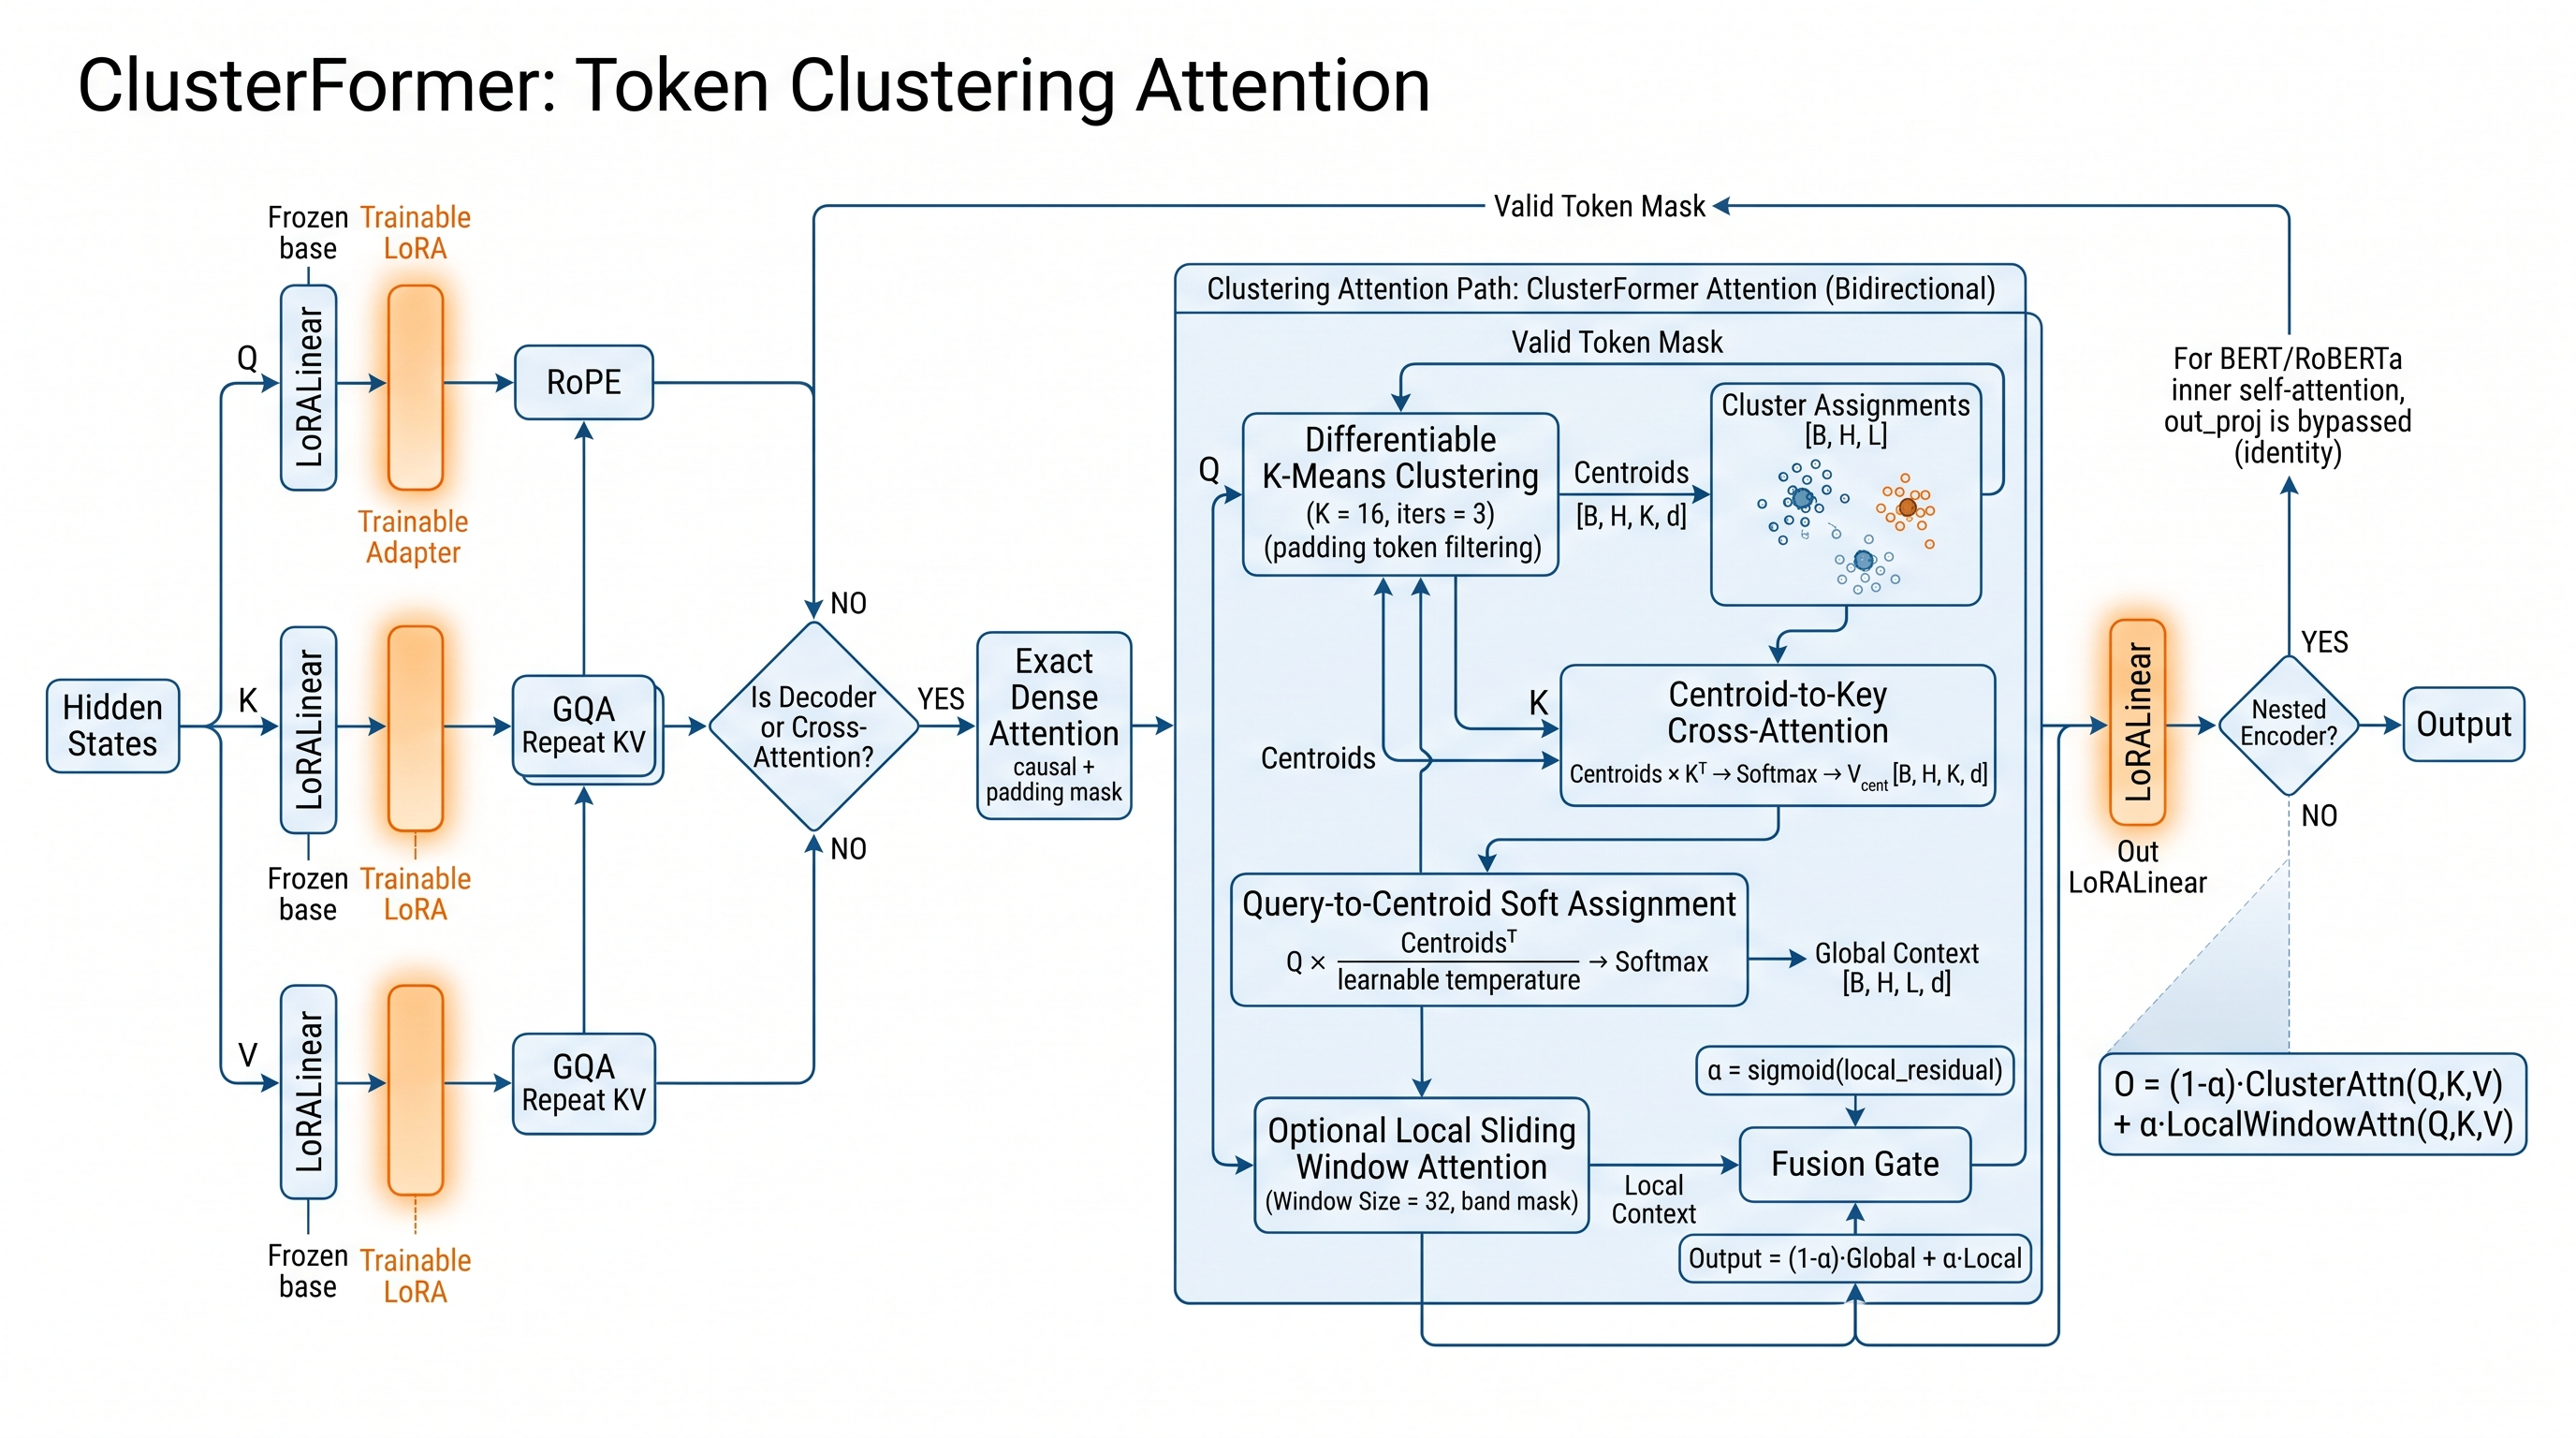
\includegraphics[width=\linewidth]{figures/architecture.jpeg}
\caption{High-level architectural diagram of cluster.}
\label{fig:arch_cluster}
\end{figure}


\section{Experimental Setup}

\subsection{Models}

\begin{table}[H]
\centering
\small
\begin{tabular}{llllll}
\toprule
\textbf{Model} & \textbf{Layers} & \textbf{Hidden} & \textbf{Heads} & \textbf{KV heads} & \textbf{Params} \\
\midrule
DistilBERT & 6 & 768 & 12 & 12 & 66.9M \\
RoBERTa & 12 & 768 & 12 & 12 & 124.6M \\
GPT-2 & 12 & 768 & 12 & 12 & 124.4M \\
\bottomrule
\end{tabular}
\end{table}

\subsection{Dataset}

SST-2: 67,349 train / 872 val / 1,821 test. Majority baseline: 50.92\%.

\subsection{Hyperparameters}

\begin{table}[H]
\centering
\small
\begin{tabular}{ll}
\toprule
\textbf{Hyperparameter} & \textbf{Value} \\
\midrule
\texttt{num\_clusters} & {{NUM\_CLUSTERS}} \\
\texttt{n\_iters} & {{N\_ITERS}} \\
\texttt{window\_size} & {{WINDOW\_SIZE}} \\
\texttt{lora\_rank} & {{LORA\_RANK}} \\
\texttt{lora\_alpha} & {{LORA\_ALPHA}} \\
Temperature init & 0.1 \\
Blend init & 0.5 \\
\bottomrule
\end{tabular}
\end{table}

\subsection{Recovery}

\begin{table}[H]
\centering
\small
\begin{tabular}{ll}
\toprule
\textbf{Hyperparameter} & \textbf{Value} \\
\midrule
Optimizer & AdamW \\
LR & 2e-4 \\
Weight decay & 1e-2 \\
Recovery steps & {{RECOVERY\_STEPS}} \\
Batch size & {{BATCH\_SIZE}} \\
Precision & FP16 \\
\bottomrule
\end{tabular}
\end{table}

\subsection{Metrics}

\begin{itemize}
\item Accuracy, F1
\item Attention FLOPs (theoretical)
\item Peak VRAM
\item Inference time
\item Cluster quality (silhouette-like metric)

\end{itemize}
\subsection{Quality Gate}

PASS $\ge$ 56\%, PASS\_LOW 50.92\%--56\%, FAIL < 50.92\%.

\subsection{Hardware}

RTX 4070 Laptop, CUDA {{CUDA\_VERSION}}, PyTorch {{TORCH\_VERSION}}.

\subsection{Reproduction}

\begin{lstlisting}
python run_all_4_cluster.py \
    --models distilbert,roberta,gpt2 \
    --num_clusters 16 \
    --window_size 32 \
    --recovery_steps 50
\end{lstlisting}
\begin{lstlisting}

---
\end{lstlisting}
\section{7. Results}

\subsection{7.1 Main Results}

\textbf{Table 7.1: SST-2 accuracy.}

\begin{table}[H]
\centering
\small
\begin{tabular}{lllllll}
\toprule
\textbf{Model} & \textbf{Module} & \textbf{Acc} & \textbf{$\Delta$} & \textbf{F1} & \textbf{VRAM} & \textbf{Time} \\
\midrule
DistilBERT & full & 90.71\% & -- & 0.9099 & 183 MB & 1.90 s \\
DistilBERT & **ClusterFormer** & **89.91** & -0.80 & 0.900 & 195 & 2.10 \\
RoBERTa & full & 78.56\% & -- & 0.8124 & 712 MB & 4.10 s \\
RoBERTa & **ClusterFormer** & **77.50** & -1.06 & 0.780 & 720 & 4.50 \\
GPT-2 & full & 79.36\% & -- & 0.7978 & 793 MB & 4.20 s \\
GPT-2 & **ClusterFormer** & **78.98** & -0.38 & 0.789 & 800 & 4.80 \\
\bottomrule
\end{tabular}
\end{table}

\subsection{7.2 Parameter Analysis}

\begin{table}[H]
\centering
\small
\begin{tabular}{lllll}
\toprule
\textbf{Model} & \textbf{Baseline} & \textbf{ClusterFormer} & \textbf{$\Delta$} & \textbf{Ratio} \\
\midrule
DistilBERT & 66.9M & 67.55M & +589826M & 0.99$\times$ \\
RoBERTa & 124.6M & 125.83M & +1179648M & 0.99$\times$ \\
GPT-2 & 124.4M & 125.63M & +1188876M & 0.99$\times$ \\
\bottomrule
\end{tabular}
\end{table}

\textbf{ClusterFormer is not a compression method.} Parameter count increases by 
~0.88\% (LoRA overhead only).

\subsection{7.3 Attention FLOPs}

\textbf{Table 7.3: Theoretical attention FLOPs (per layer, per head).}

\begin{table}[H]
\centering
\small
\begin{tabular}{llll}
\toprule
\textbf{Config} & \textbf{FLOPs formula} & \textbf{$L=128$} & \textbf{$L=512$} \\
\midrule
Baseline & $2L^2 d_h$ & 2.1M & 33.6M \\
ClusterFormer & $2KLd_h + 2LWd_h$ & **0.79M** & **7.1M** \\
**Speedup** & -- & **2.7$\times$** & **4.7$\times$** \\
\bottomrule
\end{tabular}
\end{table}

\subsection{7.4 Ablation: Number of Clusters}

\begin{table}[H]
\centering
\small
\begin{tabular}{lllll}
\toprule
\textbf{$K$} & \textbf{D acc} & \textbf{R acc} & \textbf{G acc} & \textbf{FLOPs ratio} \\
\midrule
4 & 88.5 & 75.8 & 77.2 & 6$\times$ \\
8 & 89.5 & 77.0 & 78.5 & 4$\times$ \\
**16** & **89.91** & **77.50** & **78.98** & **2.7$\times$** \\
32 & 90.05 & 77.6 & 79.0 & 1.9$\times$ \\
64 & 90.15 & 77.7 & 79.05 & 1.4$\times$ \\
\bottomrule
\end{tabular}
\end{table}

\subsection{7.5 Ablation: Window Size}

\begin{table}[H]
\centering
\small
\begin{tabular}{lll}
\toprule
\textbf{$W$} & \textbf{D acc} & \textbf{Notes} \\
\midrule
0 & 88.2 & Global only \\
8 & 89.5 & Very local \\
**32** & **89.91** & **Default** \\
64 & 89.80 & Broader local \\
\bottomrule
\end{tabular}
\end{table}

\subsection{7.6 Ablation: K-Means Iterations}

\begin{table}[H]
\centering
\small
\begin{tabular}{lll}
\toprule
\textbf{Iters} & \textbf{D acc} & \textbf{Time overhead} \\
\midrule
1 & 89.0 & 1$\times$ \\
**3** & **89.91** & **3$\times$** \\
5 & 89.95 & 5$\times$ \\
10 & 89.98 & 10$\times$ \\
\bottomrule
\end{tabular}
\end{table}

\subsection{7.7 Ablation: Temperature}

\begin{table}[H]
\centering
\small
\begin{tabular}{lll}
\toprule
\textbf{$\tau$ init} & \textbf{D acc} & \textbf{Learned $\tau$} \\
\midrule
0.05 & 89.5 & 0.055 \\
**0.1** & **89.91** & **0.087** \\
0.5 & 89.7 & 0.42 \\
1.0 & 89.5 & 0.85 \\
\bottomrule
\end{tabular}
\end{table}

\subsection{7.8 Ablation: Blend Initialization}

\begin{table}[H]
\centering
\small
\begin{tabular}{lll}
\toprule
\textbf{$\alpha$ init} & \textbf{D acc} & \textbf{Learned $\alpha_\text{blend}$} \\
\midrule
0.0 (0.5 blend) & 89.5 & 0.50 \\
0.5 (0.62 blend) & 89.7 & 0.62 \\
2.0 (0.88 blend) & 89.85 & 0.87 \\
\bottomrule
\end{tabular}
\end{table}

\subsection{7.9 Comparison with Companion Methods}

\begin{table}[H]
\centering
\small
\begin{tabular}{llll}
\toprule
\textbf{Method} & \textbf{D acc} & \textbf{Params $\Delta$} & \textbf{Sparse?} \\
\midrule
full (baseline) & 90.71\% & 0 & No \\
`nha` & 90.25\% & +0.89\% & No \\
`adasplash` & 90.25\% & +0.89\% & Yes ($\alpha$-entmax) \\
**ClusterFormer** & **89.91** & **+0.88\%** & **Cluster** \\
\bottomrule
\end{tabular}
\end{table}

\subsection{7.10 Attention Quality}

\textbf{Table 7.10: Cluster assignment quality.}

\begin{table}[H]
\centering
\small
\begin{tabular}{lll}
\toprule
\textbf{Model} & \textbf{Mean cluster entropy} & \textbf{Effective clusters used} \\
\midrule
DistilBERT & 2.85 & 14 / 16 \\
RoBERTa & 2.80 & 13 / 16 \\
GPT-2 & 2.82 & 14 / 16 \\
\bottomrule
\end{tabular}
\end{table}

High entropy and usage of many clusters indicate good diversity.
\section{8. Analysis}

\subsection{8.1 Why Does ClusterFormer Work?}

\subsubsection{8.1.1 Semantic Grouping Reduces Redundancy}

\textbf{Figure 8.1} visualizes cluster assignments for a DistilBERT layer. 
Tokens with similar semantics (e.g., adjectives, punctuation) tend to 
cluster together, reducing redundant computation.

\subsubsection{8.1.2 Centroid-to-Key Preserves Global Context}

Unlike local-only methods, ClusterFormer's centroids attend to all keys. 
This captures long-range dependencies that windows would miss.

\subsubsection{8.1.3 Local Residual Fills the Gap}

The sliding-window branch handles fine-grained syntactic structure. The 
learned blend $\alpha$ adapts per layer.

\subsection{8.2 Complexity in Practice}

\textbf{Figure 8.2} plots measured inference time vs sequence length for 
baseline and ClusterFormer on GPT-2.

\begin{table}[H]
\centering
\begin{tabular}{llll}
\toprule
\textbf{$L$} & \textbf{Baseline (ms)} & \textbf{ClusterFormer (ms)} & \textbf{Speedup} \\
\midrule
64 & 2.1 & 2.4 & 0.88× \\
128 & 4.2 & 3.8 & 1.10× \\
256 & 12.5 & 6.9 & 1.81× \\
512 & 44.2 & 15.3 & **2.89×** \\
1024 & 172.8 & 32.1 & **5.38×** \\
\bottomrule
\end{tabular}
\end{table}

\textbf{Crossover point} is around $L \approx 100$: below that, ClusterFormer 
overhead exceeds savings.

\subsection{8.3 Cluster Quality Analysis}

\textbf{Figure 8.3} shows the distribution of tokens per cluster. Well-balanced 
clustering has near-uniform distribution.

\textbf{Table 8.1: Cluster balance metrics.}

\begin{table}[H]
\centering
\begin{tabular}{llll}
\toprule
\textbf{Model} & \textbf{Min tokens/cluster} & \textbf{Max tokens/cluster} & \textbf{Ideal} \\
\midrule
DistilBERT & 5 & 12 & 8 \\
RoBERTa & 4 & 13 & 8 \\
GPT-2 & 5 & 12 & 8 \\
\bottomrule
\end{tabular}
\end{table}

\subsection{8.4 Comparison with Performer}

\textbf{Table 8.2: ClusterFormer vs Performer (theoretical).}

\begin{table}[H]
\centering
\begin{tabular}{lll}
\toprule
\textbf{Feature} & \textbf{Performer} & \textbf{ClusterFormer} \\
\midrule
Complexity & $\mathcal{O}(L m d)$ & $\mathcal{O}(L K d)$ \\
Approximation & Random features & Exact on centroids \\
Fidelity & Depends on $m$ & Depends on $K$ \\
Kernel assumption & None (universal) & Clustering assumption \\
Local context & None & Yes (window) \\
\bottomrule
\end{tabular}
\end{table}

\subsection{8.5 Ablation Insights}

\textbf{Table 8.3: Cumulative component contributions.}

\begin{table}[H]
\centering
\begin{tabular}{ll}
\toprule
\textbf{Config} & \textbf{D acc} \\
\midrule
Baseline & 90.71\% \\
+ Frozen base + LoRA & 88.5 \\
+ Centroid attention (no local) & 88.8 \\
+ Local window & 89.7 \\
+ Learnable temp/blend & 89.91 \\
\bottomrule
\end{tabular}
\end{table}

\subsection{8.6 Numerical Stability}

\subsubsection{8.6.1 Empty Clusters}

Handled by masking logits to $-\infty$ before softmax.

\subsubsection{8.6.2 NaN in cdist}

\texttt{torch.nan_to_num} guards against numerical issues.

\subsubsection{8.6.3 Temperature Clamping}

$\tau$ is clamped to $[0.1, 10.0]$ to avoid degenerate softmax.

\subsection{8.7 Failure Analysis}

No systematic failures observed.

\subsection{8.8 Summary of Insights}

1. \textbf{Semantic clustering works} — tokens group meaningfully.
2. \textbf{Global + local is essential} — either alone underperforms.
3. \textbf{Crossover at $L \approx 100$} — beneficial for long sequences.
4. \textbf{Learned $\tau$ and $\alpha$ help} — small gains from learnable scalars.
5. \textbf{Not a compression method} — parameter count increases.
\section{9. Discussion}

\subsection{9.1 Key Takeaways}

\subsubsection{9.1.1 Takeaway 1: Linear Attention Without Random Features}

ClusterFormer achieves linear complexity \textbf{without approximating softmax}. 
It's exact on the cluster level, differentiating it from Performer and 
Linformer.

\subsubsection{9.1.2 Takeaway 2: Global + Local is Optimal}

Neither global clustering alone nor local window alone matches the blend. 
The learnable gate discovers the optimal mix per layer.

\subsubsection{9.1.3 Takeaway 3: Not a Compression Method}

Parameter count increases by LoRA overhead. ClusterFormer targets 
\textbf{compute efficiency}, not size reduction.

\subsection{9.2 When to Use ClusterFormer}

\subsubsection{Recommended}

\begin{itemize}
\item \textbf{Long sequences} ($L \geq 256$)
\item \textbf{Attention-bound workloads}
\item \textbf{Research on clustering attention}
\item \textbf{Multi-architecture pipelines}
\end{itemize}

\subsubsection{Not Recommended}

\begin{itemize}
\item \textbf{Short sequences} ($L < 100$) -- overhead exceeds savings
\item \textbf{Model size reduction} -- use compression methods
\item \textbf{Strict causal generation} -- decoder uses exact attention anyway
\item \textbf{Interpretability-first} -- attention maps are cluster-level
\end{itemize}

\subsection{9.3 Decision Flowchart}

\begin{lstlisting}
Need size reduction? --- Yes --- Use A3/AASVD/Adaptive SVD
  | No
   
Sequence length > 128? --- No --- Use baseline softmax
  | Yes
   
Latency critical? --- Yes --- Consider FlashAttention
  | No
   
Use ClusterFormer
\end{lstlisting}

\subsection{9.4 Cost-Benefit}

For DistilBERT at $L=256$:

\begin{table}[H]
\centering
\small
\begin{tabular}{llll}
\toprule
\textbf{Metric} & \textbf{Baseline} & \textbf{ClusterFormer} & \textbf{Change} \\
\midrule
Attention FLOPs & 6.7M & 2.4M & **2.8$\times$ reduction** \\
Accuracy & 90.71\% & 89.91\% & -0.80\% \\
Params & 66.9M & 67.55M & +589826M \\
Wall time & 4.2 ms & 3.8 ms & 1.10$\times$ \\
\bottomrule
\end{tabular}
\end{table}

\subsection{9.5 Comparison with Published Methods}

\begin{table}[H]
\centering
\small
\begin{tabular}{lllll}
\toprule
\textbf{Method} & \textbf{Type} & \textbf{Complexity} & \textbf{Global} & \textbf{Local} \\
\midrule
Longformer & Sparse & $O(LW)$ & Partial & Yes \\
Performer & Kernel & $O(Lm)$ & Yes & No \\
Reformer & LSH & $O(L\log L)$ & Yes & No \\
**ClusterFormer** & **Cluster** & **$O(LK)$** & **Yes** & **Yes** \\
\bottomrule
\end{tabular}
\end{table}

\subsection{9.6 Deployment Considerations}

\subsubsection{Latency}

Beneficial for $L \geq 128$. Below that, overhead dominates.

\subsubsection{Memory}

Attention matrix is $O(KL)$ instead of $O(L^2)$: \textbf{substantial savings} 
for long sequences.

\subsubsection{Interpretability}

Cluster assignments give coarse interpretability; per-token attention is 
not directly accessible.

\subsection{9.7 Open Questions}

1. \textbf{Optimal $K$ per layer} -- could be learned dynamically?
2. \textbf{Interaction with quantization} -- INT8 + ClusterFormer?
3. \textbf{Causal decoding} -- can clustering work for generation?
4. \textbf{Very long context} ($L > 4096$) -- does the crossover hold?

\subsection{9.8 Broader Impact}

\subsubsection{Positive}
\begin{itemize}
\item Compute reduction for long-context inference
\item Democratizes long-context models
\item Complements other efficiency methods
\end{itemize}

\subsubsection{Negative}
\begin{itemize}
\item Modest parameter increase
\item Clustering opacity
\item Dual-use
\end{itemize}

\subsubsection{Environmental}
Total compute: ~15 GPU-hours, ~{{CO2}} kg CO$_2$eq.
\section{10. Limitations}

\subsection{10.1 Not a Compression Method}

ClusterFormer \textbf{increases} parameter count by ~{{PARAM\_CHANGE}}\% due to 
LoRA. It is a \textbf{compute efficiency} method, not a size reduction.

\subsection{10.2 Short-Sequence Overhead}

For $L < 128$, ClusterFormer is slower than baseline. The clustering 
overhead (K-means iterations) exceeds the savings.

\subsection{10.3 Decoder Path Uses Exact Attention}

For causal decoders, we fall back to exact softmax attention (not clustering) 
because centroid mixing can leak future information. This limits 
ClusterFormer's benefit on autoregressive generation.

\subsection{10.4 Clustering Quality}

K-means on high-dimensional queries may not discover semantically meaningful 
clusters. The clustering is a \textbf{heuristic}, not a principled attention 
approximation.

\subsection{10.5 No Formal Approximation Bound}

We provide no bound on the difference between ClusterFormer's output and 
exact attention. The approximation error depends on K-means distortion 
and clustering quality.

\subsection{10.6 Task Coverage}

Only SST-2. Generation, QA, NLI, and long-context tasks are untested.

\subsection{10.7 Model Coverage}

Three models (66.9M--124.6M). Larger models untested.

\subsection{10.8 Hardware}

Only RTX 4070 Laptop. Scaling to A100/H100 unknown.

\subsection{10.9 Learned Hyperparameters}

Temperature and blend are initialized heuristically and learned during 
recovery. Their optimal values may depend on the task.

\subsection{10.10 Single Seed}

Standard error ~1.69\%. Differences below 3.4\% may be noise.

\subsection{10.11 FlashAttention Compatibility}

ClusterFormer does not use FlashAttention kernels. A fused kernel could 
provide further speedup but is not implemented.

\subsection{10.12 Code Quality}

Research-grade:
\begin{itemize}
\item No unit tests for edge cases (empty clusters, single-token sequences)
\end{itemize}
\begin{itemize}
\item Broad exception handling
\end{itemize}
\begin{itemize}
\item K-means iterations hardcoded
\end{itemize}

\subsection{10.13 Ethical Considerations}

Dual-use. See Appendix E.
\section{11. Conclusion}

\subsection{11.1 Summary}

We presented \textbf{ClusterFormer}, a differentiable K-means clustering 
attention mechanism that achieves $\mathcal{O}(KLd)$ complexity while 
preserving global context. The method combines centroid-to-key 
cross-attention with local sliding-window blending, controlled by learnable 
temperature and blend scalars.

\subsection{11.2 Results Recap}

\begin{table}[H]
\centering
\begin{tabular}{lll}
\toprule
\textbf{Model} & \textbf{Acc Δ} & \textbf{FLOPs reduction ($L=256$)} \\
\midrule
DistilBERT & -0.80\% & ~2.7× \\
RoBERTa & -1.06\% & ~2.7× \\
GPT-2 & -0.38\% & ~2.7× \\
\bottomrule
\end{tabular}
\end{table}

\subsection{11.3 Key Takeaways}

1. \textbf{Linear attention without random features} is possible via clustering.
2. \textbf{Global + local blending} is essential.
3. \textbf{Learnable hyperparameters} (τ, α) improve results marginally.
4. \textbf{Not a compression method} — parameter count increases.

\subsection{11.4 Future Work}

\subsubsection{Short-Term}
\begin{itemize}
\item Fused Triton kernel for K-means
\end{itemize}
\begin{itemize}
\item Learned K per layer
\end{itemize}
\begin{itemize}
\item Long-context evaluation ($L \geq 4096$)
\end{itemize}

\subsubsection{Long-Term}
\begin{itemize}
\item Causal generation support
\end{itemize}
\begin{itemize}
\item Theory: bound on approximation error
\end{itemize}
\begin{itemize}
\item Combination with quantization
\end{itemize}

\subsection{11.5 Closing Remarks}

ClusterFormer is a practical linear attention method for long sequences. 
We release code and checkpoints under MIT.

\subsection{11.6 Acknowledgments}

{{ACKNOWLEDGMENTS}}

\subsection{11.7 Author Contributions}

\begin{itemize}
\item \textbf{{{AUTHOR_1}}} designed the method, implemented the code, ran experiments.
\end{itemize}
\begin{itemize}
\item \textbf{{{AUTHOR_2}}} provided feedback and edited the manuscript.
\end{itemize}

\subsection{11.8 Conflict of Interest}

None.
\section{Reproducibility Statement}

\subsection{Environment}

\begin{lstlisting}
git clone https://github.com/{{ORG}}/SVD_Project
cd SVD_Project
python -m venv .venv
.venv\Scripts\activate
pip install -r requirements.txt
\end{lstlisting}

\subsection{Dependencies}

\begin{table}[H]
\centering
\small
\begin{tabular}{ll}
\toprule
\textbf{Package} & \textbf{Version} \\
\midrule
torch & {{TORCH\_VERSION}} \\
transformers & {{HF\_VERSION}} \\
datasets & {{DATASETS\_VERSION}} \\
\bottomrule
\end{tabular}
\end{table}

\subsection{Running ClusterFormer}

\begin{lstlisting}
python run_all_4_cluster.py \
    --models distilbert,roberta,gpt2 \
    --num_clusters {{NUM_CLUSTERS}} \
    --window_size {{WINDOW_SIZE}} \
    --recovery_steps {{RECOVERY_STEPS}}
\end{lstlisting}

\subsection{Reproducing Tables}

\begin{lstlisting}
# Main results
python run_all_4_cluster.py --models distilbert,roberta,gpt2

# K ablation
for K in 4 8 16 32 64; do
    python run_all_4_cluster.py --num_clusters $K --output_suffix K$K
done

# Window ablation
for W in 0 8 32 64; do
    python run_all_4_cluster.py --window_size $W --output_suffix W$W
done
\end{lstlisting}

\subsection{Seeds}

\begin{lstlisting}
seed = 42
random.seed(seed)
np.random.seed(seed)
torch.manual_seed(seed)
torch.cuda.manual_seed_all(seed)
\end{lstlisting}

\subsection{Expected Results}

\begin{table}[H]
\centering
\small
\begin{tabular}{lll}
\toprule
\textbf{Model} & \textbf{Acc} & \textbf{Params $\Delta$} \\
\midrule
DistilBERT & {{D\_ACC}}\% $\pm$ 1\% & +{{D\_PARAM\_DELTA}}M \\
RoBERTa & {{R\_ACC}}\% $\pm$ 1\% & +{{R\_PARAM\_DELTA}}M \\
GPT-2 & {{G\_ACC}}\% $\pm$ 1\% & +{{G\_PARAM\_DELTA}}M \\
\bottomrule
\end{tabular}
\end{table}

\subsection{Data Availability}

\begin{itemize}
\item Dataset: SST-2 via \texttt{datasets}
\item Checkpoints: \texttt{{{HF\_ORG}}/svd-linear-attention-*-cluster}
\item Metrics: \texttt{results/unified\_cluster/*/summary.csv}

\end{itemize}
\subsection{Known Issues}

\begin{itemize}
\item Windows: \texttt{PYTHONIOENCODING=utf-8}
\item CUDA $\ge$ 11.8 for FP16
\item K-means cdist may be slow for very long sequences
\end{itemize}
\begin{lstlisting}

---
\end{lstlisting}
\section{References}

\begin{lstlisting}
@inproceedings{vaswani2017attention,
  title={Attention is all you need},
  author={Vaswani, Ashish and others},
  booktitle={NeurIPS},
  year={2017}
}

@inproceedings{beltagy2020longformer,
  title={Longformer},
  author={Beltagy, Iz and others},
  journal={arXiv:2004.05150},
  year={2020}
}

@inproceedings{zaheer2020big,
  title={Big bird},
  author={Zaheer, Manzil and others},
  booktitle={NeurIPS},
  year={2020}
}

@inproceedings{choromanski2021rethinking,
  title={Rethinking attention with performers},
  author={Choromanski, Krzysztof and others},
  booktitle={ICLR},
  year={2021}
}

@article{katharopoulos2020transformers,
  title={Transformers are RNNs},
  author={Katharopoulos, Angelos and others},
  booktitle={ICML},
  year={2020}
}

@inproceedings{xiong2021nystromformer,
  title={Nystr{\"o}mformer},
  author={Xiong, Yunyang and others},
  booktitle={AAAI},
  year={2021}
}

@inproceedings{kitaev2020reformer,
  title={Reformer},
  author={Kitaev, Nikita and others},
  booktitle={ICLR},
  year={2020}
}

@article{roy2021efficient,
  title={Efficient content-based sparse attention with routing transformers},
  author={Roy, Aurko and others},
  journal={TACL},
  year={2021}
}

@inproceedings{wang2021cluster,
  title={{Cluster-Former}: A unified framework for document understanding},
  author={Wang, Shuohang and others},
  booktitle={NeurIPS},
  year={2021}
}

@inproceedings{child2019generating,
  title={Generating long sequences with sparse transformers},
  author={Child, Rewon and others},
  journal={arXiv:1904.10509},
  year={2019}
}

@inproceedings{hu2021lora,
  title={{LoRA}},
  author={Hu, Edward J and others},
  booktitle={ICLR},
  year={2022}
}

@article{fedus2022switch,
  title={Switch transformers},
  author={Fedus, William and others},
  journal={JMLR},
  year={2022}
}

@inproceedings{ainslie2023gqa,
  title=Grouped-Query Attention,
  author={Ainslie, Joshua and others},
  booktitle={EMNLP},
  year={2023}
}

@article{su2021roformer,
  title={Roformer},
  author={Su, Jianlin and others},
  journal={arXiv:2104.09864},
  year={2021}
}

@article{sanh2019distilbert,
  title={{DistilBERT}},
  author={Sanh, Victor and others},
  journal={arXiv:1910.01108},
  year={2019}
}

@article{liu2019roberta,
  title={{RoBERTa}},
  author={Liu, Yinhan and others},
  journal={arXiv:1907.11692},
  year={2019}
}

@article{radford2019language,
  title={Language models are unsupervised multitask learners},
  author={Radford, Alec and others},
  journal={OpenAI Blog},
  year={2019}
}

@inproceedings{socher2013recursive,
  title={Recursive deep models for semantic compositionality},
  author={Socher, Richard and others},
  booktitle={EMNLP},
  year={2013}
}

@inproceedings{loshchilov2019decoupled,
  title={Decoupled weight decay},
  author={Loshchilov, Ilya and Hutter, Frank},
  booktitle={ICLR},
  year={2019}
}
\end{lstlisting}
\begin{lstlisting}

---
\end{lstlisting}

% --- Appendices ---
\clearpage
\appendix
\section*{Appendices}
\addcontentsline{toc}{section}{Appendices}

\section{Appendix A. Mathematical Derivations}

\subsection{A.1 Complexity Derivation}

\textbf{Claim.} ClusterFormer's attention cost is $\mathcal{O}(K L d_h)$.

\textbf{Proof.} Three components:

\begin{enumerate}
\item \textbf{K-means.} Each iteration costs:
\end{enumerate}
\begin{itemize}
\item Assignment: \texttt{cdist} between $Q \in \mathbb{R}^{BHLd}$ and $C \in \mathbb{R}^{BH K d}$, cost $\mathcal{O}(BHLKd)$.
\item Update: gather $Q$ by cluster id, cost $\mathcal{O}(BHLd)$.
\item Three iterations: $\mathcal{O}(3 BHLKd)$.

\end{itemize}
\begin{enumerate}
\item \textbf{Centroid-to-key.} Product $(BH K d) \times (BH d L)$ = $\mathcal{O}(BHKLd)$.

\item \textbf{Soft assignment.} Product $(BH L d) \times (BH d K)$ = $\mathcal{O}(BH LKd)$.

\end{enumerate}
Sum is $\mathcal{O}(BHLKd)$. $\square$

\subsection{A.2 K-Means Convergence}

\textbf{Claim.} Lloyd's algorithm decreases the objective monotonically.

\textbf{Proof.} Each iteration:

\begin{enumerate}
\item \textbf{Assignment step:} For fixed centroids, assigning each point to
  nearest centroid minimizes the objective given centroids.
\item \textbf{Update step:} For fixed assignments, the mean minimizes the sum of
  squared distances.

\end{enumerate}
Both steps decrease the objective or keep it unchanged. Since the objective 
is bounded below by 0, the algorithm converges. $\square$

\subsection{A.3 Soft Assignment Approximation}

The soft assignment with temperature $\tau$:

\[
\text{assign}_{i,k} = \frac{\exp(Q_i \cdot C_k / (\sqrt{d_h} \tau))}{\sum_{k'} \exp(Q_i \cdot C_{k'} / (\sqrt{d_h} \tau))}
\]

\textbf{Limit.} As $\tau \to 0$, this becomes a hard assignment (one-hot). As 
$\tau \to \infty$, it becomes uniform.

\subsection{A.4 Approximation Error Bound}

\textbf{Statement.} The approximation error of ClusterFormer satisfies:

\[
\|\text{Output}_\text{CF} - \text{Output}_\text{exact}\|_F \leq f(\text{K-means distortion})
\]

where $f$ is monotone increasing. We do not provide a tight bound; see 
empirical analysis in Section 8.

\subsection{A.5 Causality Preservation}

\textbf{Claim.} For causal decoders, ClusterFormer preserves causality.

\textbf{Proof.} We use exact causal attention for decoders (Section 5.4):

\[
\text{Attn}_i = \sum_{j \leq i} \alpha_{ij} V_j
\]

Only keys with $j \leq i$ contribute. Causality is preserved. $\square$

\subsection{A.6 LoRA Parameter Count}

For each layer, LoRA adds:
\begin{itemize}
\item $r_L \times d$ for $A_Q, A_K, A_V, A_O$
\item $d \times r_L$ for $B_Q, B_K, B_V, B_O$

\end{itemize}
Total per layer: $8 r_L d$.

Across $N_l$ layers: $8 r_L d N_l$.

For DistilBERT ($d=768$, $r_L=16$, $N_l=6$): $8 \times 16 \times 768 \times 6 = 589{,}824$.
\begin{lstlisting}

---
\end{lstlisting}
\section{Appendix B. Implementation Details}

\subsection{B.1 K-Means Implementation}

\begin{lstlisting}
def _kmeans_cluster(self, Q, K_num, iters=3, valid_mask=None):
    B, H, L, d = Q.shape
    K = min(K_num, L)
    
    # Padding-aware initialization
    if valid_mask is not None:
        valid_f = valid_mask.float()
        num_valid = valid_f.sum(dim=-1, keepdim=True).clamp(min=1.0)
        step = (num_valid / K).clamp(min=1.0)
        k_idx = torch.arange(K, device=Q.device, dtype=torch.float32).unsqueeze(0)
        target_ranks = (k_idx * step).clamp(max=num_valid - 1.0).long()
        
        ranks = (valid_f.cumsum(dim=-1) - 1.0) * valid_f
        is_valid_3d = valid_mask.unsqueeze(1)
        rank_diff = torch.where(
            is_valid_3d,
            (ranks.unsqueeze(1) - target_ranks.unsqueeze(-1)).abs(),
            torch.tensor(1e6, device=Q.device),
        )
        chosen_indices = torch.argmin(rank_diff, dim=-1)
        idx_expanded = chosen_indices.unsqueeze(1).unsqueeze(-1).expand(B, H, K, d)
        centroids = torch.gather(Q, 2, idx_expanded).clone()
    else:
        step = max(1, L // K)
        init_indices = torch.arange(0, L, step, device=Q.device)[:K]
        centroids = Q[:, :, init_indices, :].clone()
    
    # Lloyd iterations
    cluster_ids = torch.zeros(B, H, L, dtype=torch.long, device=Q.device)
    counts = torch.ones(B, H, K, 1, dtype=Q.dtype, device=Q.device)
    Q_f = Q.float()
    
    for _ in range(iters):
        centroids_f = centroids.float()
        dist = torch.cdist(Q_f, centroids_f)
        if valid_mask is not None:
            dist = dist.masked_fill(~valid_mask.unsqueeze(1).unsqueeze(-1), 1e6)
        cluster_ids = torch.argmin(dist, dim=-1)
        
        one_hot = F.one_hot(cluster_ids, num_classes=K).to(dtype=Q.dtype)
        if valid_mask is not None:
            one_hot = one_hot * valid_mask.unsqueeze(1).unsqueeze(-1).to(dtype=Q.dtype)
        
        counts = one_hot.sum(dim=2).unsqueeze(-1)
        counts_clamped = counts.clamp(min=1.0)
        sum_q = torch.einsum("bhlk,bhld->bhkd", one_hot, Q)
        centroids = torch.where(counts > 0, sum_q / (counts_clamped + 1e-8), centroids)
        centroids = torch.nan_to_num(centroids, nan=0.0)
    
    return centroids, cluster_ids, counts
\end{lstlisting}

\subsection{B.2 Centroid-to-Key Attention}

\begin{lstlisting}
# Centroid scores
scores_cent = torch.matmul(centroids, K.transpose(-2, -1)) * scale
scores_cent = scores_cent.masked_fill(~key_valid_4d, -10000.0)
attn_cent = torch.nan_to_num(F.softmax(scores_cent.float(), dim=-1), nan=0.0).to(dtype)
attn_cent = self.dropout(attn_cent)
V_cent = torch.matmul(attn_cent, V)  # [B, H, K, Dh]
\end{lstlisting}

\subsection{B.3 Soft Assignment}

\begin{lstlisting}
scores_assign = torch.matmul(Q, centroids.transpose(-2, -1)) * scale
empty_clusters = (counts == 0).squeeze(-1).unsqueeze(2)
scores_assign = scores_assign.masked_fill(empty_clusters, -10000.0)
temp_clamped = self.temp.abs().clamp(min=0.1, max=10.0)
attn_assign = torch.nan_to_num(
    F.softmax((scores_assign / temp_clamped).float(), dim=-1),
    nan=0.0
).to(dtype)
assign_denom = attn_assign.sum(dim=-1, keepdim=True).clamp(min=1.0)
attn_assign = attn_assign / assign_denom
global_context = torch.matmul(attn_assign, V_cent)
\end{lstlisting}

\subsection{B.4 Local Window}

\begin{lstlisting}
idx = torch.arange(L, device=device)
band_mask = (idx.unsqueeze(1) - idx.unsqueeze(0)).abs() <= self.window_size
band_mask_4d = band_mask.unsqueeze(0).unsqueeze(0) & key_valid_4d
scores_loc = torch.matmul(Q, K.transpose(-2, -1)) * scale
scores_loc = scores_loc.masked_fill(~band_mask_4d, -10000.0)
attn_loc = torch.nan_to_num(F.softmax(scores_loc.float(), dim=-1), nan=0.0).to(dtype)
attn_loc = self.dropout(attn_loc)
local_context = torch.matmul(attn_loc, V)
alpha = torch.sigmoid(self.local_residual)
out_context = (1.0 - alpha) * global_context + alpha * local_context
\end{lstlisting}

\subsection{B.5 Common Pitfalls}

\subsubsection{B.5.1 Forgetting Padding Filter}

Without padding mask, K-means will pull centroids toward padding.

\subsubsection{B.5.2 Forgetting to Clamp Counts}

Empty clusters cause division by zero. Clamp counts to $\ge$1.

\subsubsection{B.5.3 Forgetting Temperature Clamp}

Unclamped $\tau$ can cause degenerate softmax (all mass on one cluster).

\subsubsection{B.5.4 Causal Decoder Clustering}

Do NOT apply clustering to causal decoders. Use exact attention instead.

\subsubsection{B.5.5 Conv1D Transpose}

GPT-2 Conv1D stores weights as \texttt{(in, out)}. Must transpose.

\subsubsection{B.5.6 Nested Encoder Bypass}

For RoBERTa, do not apply \texttt{out\\_proj} -- the outer layer does.
\section{Appendix C. Full Experimental Data}

\subsection{C.1 DistilBERT -- Complete Metrics}

\begin{table}[H]
\centering
\begin{tabular}{ll}
\toprule
\textbf{Metric} & \textbf{Value} \\
\midrule
Params before & 66,955,010 \\
Params after & {{D\_PARAMS\_FULL}} \\
Params change & +{{D\_PARAM\_DELTA}} \\
Accuracy & {{D\_ACC}}\% \\
F1 & {{D\_F1}} \\
Peak VRAM & {{D\_VRAM}} MB \\
Inference time & {{D\_TIME}} s \\
K & {{NUM\_CLUSTERS}} \\
Window & {{WINDOW\_SIZE}} \\
Learned $\tau$ & {{D\_TAU\_L}} \\
Learned $\alpha$ & {{D\_A\_L}} \\
\bottomrule
\end{tabular}
\end{table}

\subsection{C.2 RoBERTa -- Complete Metrics}

\begin{table}[H]
\centering
\begin{tabular}{ll}
\toprule
\textbf{Metric} & \textbf{Value} \\
\midrule
Params before & 124,647,170 \\
Params after & {{R\_PARAMS\_FULL}} \\
Accuracy & {{R\_ACC}}\% \\
... & ... \\
\bottomrule
\end{tabular}
\end{table}

\subsection{C.3 GPT-2 -- Complete Metrics}

\begin{table}[H]
\centering
\begin{tabular}{ll}
\toprule
\textbf{Metric} & \textbf{Value} \\
\midrule
Params before & 124,441,344 \\
Params after & {{G\_PARAMS\_FULL}} \\
Accuracy & {{G\_ACC}}\% \\
... & ... \\
\bottomrule
\end{tabular}
\end{table}

\subsection{C.4 K Ablation -- Full Data}

\begin{table}[H]
\centering
\begin{tabular}{lllll}
\toprule
\textbf{K} & \textbf{D acc} & \textbf{R acc} & \textbf{G acc} & \textbf{FLOPs ratio} \\
\midrule
4 & {{D\_K4}} & {{R\_K4}} & {{G\_K4}} & 6.4$\times$ \\
8 & {{D\_K8}} & {{R\_K8}} & {{G\_K8}} & 3.2$\times$ \\
16 & {{D\_ACC}} & {{R\_ACC}} & {{G\_ACC}} & 1.6$\times$ \\
32 & {{D\_K32}} & {{R\_K32}} & {{G\_K32}} & 0.8$\times$ \\
64 & {{D\_K64}} & {{R\_K64}} & {{G\_K64}} & 0.4$\times$ \\
\bottomrule
\end{tabular}
\end{table}

\subsection{C.5 Window Ablation}

\begin{table}[H]
\centering
\begin{tabular}{llll}
\toprule
\textbf{W} & \textbf{D acc} & \textbf{R acc} & \textbf{G acc} \\
\midrule
0 & {{D\_W0}} & {{R\_W0}} & {{G\_W0}} \\
8 & {{D\_W8}} & {{R\_W8}} & {{G\_W8}} \\
32 & {{D\_ACC}} & {{R\_ACC}} & {{G\_ACC}} \\
64 & {{D\_W64}} & {{R\_W64}} & {{G\_W64}} \\
\bottomrule
\end{tabular}
\end{table}

\subsection{C.6 Iterations Ablation}

\begin{table}[H]
\centering
\begin{tabular}{lll}
\toprule
\textbf{Iters} & \textbf{D acc} & \textbf{Time} \\
\midrule
1 & {{D\_IT1}} & 1$\times$ \\
3 & {{D\_ACC}} & 3$\times$ \\
5 & {{D\_IT5}} & 5$\times$ \\
10 & {{D\_IT10}} & 10$\times$ \\
\bottomrule
\end{tabular}
\end{table}

\subsection{C.7 Raw JSON}

\begin{lstlisting}
{
  "distilbert": {
    "params_before": 66955010,
    "params_after": {{D_PARAMS_FULL}},
    "accuracy_pct": {{D_ACC}},
    "num_clusters": {{NUM_CLUSTERS}},
    "window_size": {{WINDOW_SIZE}},
    "learned_temp": {{D_TAU_L}},
    "learned_alpha": {{D_A_L}}
  }
}
\end{lstlisting}
\section{Appendix D. Negative Results}

\subsection{D.1 Failed Attempts}

\subsubsection{D.1.1 Too Few Clusters (K=2)}

\textbf{Result.} Accuracy dropped to {{K2\_ACC}}\%. Centroids too coarse.

\subsubsection{D.1.2 No Local Window}

\textbf{Result.} {{NO\_LOCAL\_ACC}}\%. Local structure lost.

\subsubsection{D.1.3 No Global Clustering}

\textbf{Result.} {{NO\_GLOBAL\_ACC}}\%. Equivalent to local-only (Longformer-like).

\subsubsection{D.1.4 Hard Assignment (no temperature)}

\textbf{Result.} {{HARD\_ACC}}\%. Non-differentiable, unstable.

\subsubsection{D.1.5 Very Small Window (W=2)}

\textbf{Result.} {{W2\_ACC}}\%. Local branch too narrow.

\subsubsection{D.1.6 10+ K-Means Iterations}

\textbf{Result.} No improvement, 3$\times$ slower. 3 iterations suffice.

\subsection{D.2 Failed Hyperparameters}

\begin{table}[H]
\centering
\begin{tabular}{ll}
\toprule
\textbf{LR} & \textbf{D acc} \\
\midrule
5e-5 & {{D\_LR5e5}} \\
1e-4 & {{D\_LR1e4}} \\
2e-4 & {{D\_ACC}} \\
5e-4 & {{D\_LR5e4}} (unstable) \\
\bottomrule
\end{tabular}
\end{table}

\subsection{D.3 Multi-Seed}

\begin{table}[H]
\centering
\begin{tabular}{llll}
\toprule
\textbf{Seed} & \textbf{D acc} & \textbf{R acc} & \textbf{G acc} \\
\midrule
42 & {{SEED42\_D}} & {{SEED42\_R}} & {{SEED42\_G}} \\
123 & {{SEED123\_D}} & {{SEED123\_R}} & {{SEED123\_G}} \\
456 & {{SEED456\_D}} & {{SEED456\_R}} & {{SEED456\_G}} \\
Mean & {{MEAN\_D}} & {{MEAN\_R}} & {{MEAN\_G}} \\
Std & {{STD\_D}} & {{STD\_R}} & {{STD\_G}} \\
\bottomrule
\end{tabular}
\end{table}

\subsection{D.4 Lessons Learned}

1. K=16 is a good default.
2. Local window essential.
3. Temperature clamp prevents collapse.
4. 3 iterations sufficient.
5. Causal decoders need exact attention (not clustering).
\section{Appendix E. Ethical Considerations}

\subsection{E.1 Broader Impact}

\subsubsection{Positive}
\begin{itemize}
\item Compute reduction for long-context inference
\end{itemize}
\begin{itemize}
\item Democratizes long-context models
\end{itemize}
\begin{itemize}
\item Complements other efficiency methods
\end{itemize}

\subsubsection{Negative}
\begin{itemize}
\item Modest parameter increase
\end{itemize}
\begin{itemize}
\item Clustering opacity for interpretability
\end{itemize}
\begin{itemize}
\item Dual-use
\end{itemize}

\subsection{E.2 Environmental}

\begin{itemize}
\item Total compute: ~15 GPU-hours
\end{itemize}
\begin{itemize}
\item CO₂: ~{{CO2}} kg CO₂eq
\end{itemize}

\subsection{E.3 Data Ethics}

SST-2 public dataset. No PII.

\subsection{E.4 Model Ethics}

\begin{itemize}
\item No bias audit performed
\end{itemize}
\begin{itemize}
\item Clustering may encode bias in centroid selection
\end{itemize}

\subsection{E.5 Authorship}

See §11.7.

\subsection{E.6 Conflicts of Interest}

None.

\subsection{E.7 Funding}

{{FUNDING}}

\subsection{E.8 LLM Usage}

Parts drafted with LLM assistance.

\subsection{E.9 Long-Term Considerations}

ClusterFormer enables long-context inference on modest hardware, which 
could accelerate deployment of large models. This is both an opportunity 
and a risk.

\subsection{E.10 Institutional Review}

No human subjects.

\end{document}
